
\documentclass{beamer}
\usecolortheme{dove}
\setbeamertemplate{navigation symbols}{}
\setbeamertemplate{footline}[text line]{%
\parbox{\linewidth}{\vspace*{-8pt}\hspace{-12pt}\insertsectionnavigationhorizontal{.9\paperwidth}{}{\hfill\hfill}}}
\usepackage{amsmath,amssymb,amsfonts,amsthm, multicol, subfigure, color}
\usepackage{bm}
\usepackage{graphicx}
\usepackage{tabularx}
\usepackage{booktabs}
\usepackage{hyperref}
\usepackage{pdfpages}
\usepackage{xcolor}
\definecolor{seagreen}{RGB}{46, 139, 87}
\def\independenT#1#2{\mathrel{\rlap{$#1#2$}\mkern2mu{#1#2}}}
\newcommand\indep{\protect\mathpalette{\protect\independenT}{\perp}}
\def\log{\text{log}}
\newcommand\logit{\text{logit}}
\newcommand\iid{\stackrel{\text{iid}}{\sim}}
\newcommand\E{\text{E}}
\newcommand\V{\text{V}}
\renewcommand\P{\text{P}}
\newcommand{\Cov}{\text{Cov}}
\newcommand{\Cor}{\text{Cor}}
\newcommand\doop{\texttt{do}}
\usepackage{stackrel}
\usepackage{tikz}
\usetikzlibrary{arrows,shapes.arrows,positioning,shapes,patterns,calc}
\newcommand\slideref[1]{\vskip .1cm \tiny \textcolor{gray}{{#1}}}
\newcommand\red[1]{\color{red}#1}
\newcommand\blue[1]{\color{blue}#1}
\newcommand\gray[1]{\color{gray}#1}
\newcommand\seagreen[1]{\color{seagreen}#1}
\newcommand\purple[1]{\color{purple}#1}
\newcommand\orange[1]{\color{orange}#1}
\newcommand\black[1]{\color{black}#1}
\newcommand\white[1]{\color{white}#1}
\newcommand\teal[1]{\color{teal}#1}
\newcommand\magenta[1]{\color{magenta}#1}
\newcommand\Fuchsia[1]{\color{Fuchsia}#1}
\newcommand\BlueGreen[1]{\color{BlueGreen}#1}
\newcommand\bblue[1]{\textcolor{blue}{\textbf{#1}}}
\newcommand\bred[1]{\textcolor{red}{\textbf{#1}}}
\newcommand\bgray[1]{\textcolor{gray}{\textbf{#1}}}
\newcommand\bgreen[1]{\textcolor{seagreen}{\textbf{#1}}}
\newcommand\bref[2]{\href{#1}{\color{blue}{#2}}}
\colorlet{lightgray}{gray!40}
\pgfdeclarelayer{bg}    % declare background layer for tikz
\pgfsetlayers{bg,main} % order layers for tikz
\newcommand\mycite[1]{\begin{scriptsize}\textcolor{darkgray}{(#1)}\end{scriptsize}}
\newcommand{\tcframe}{\frame{
%\small{
\only<1|handout:0>{\tableofcontents}
\only<2|handout:1>{\tableofcontents[currentsubsection]}}
%}
}
\usepackage{verbatim}

\newcommand{\goalsframe}{\begin{frame}{Learning goals for today}
By the end of class, you will be able to
\begin{itemize}
    \item sample from a population in R
    \item write an estimator function
    \item apply the function to your sample
    \item connect sampling to the replication crisis
    \item discuss the future of sampling
 \end{itemize} 
  \vskip .2in
\end{frame}}

\newcommand{\credible}{\begin{frame}{Credible science}
\begin{enumerate}
\item replicability
\item reproducibility
\end{enumerate}
\end{frame}}

\usepackage[round]{natbib}
\bibliographystyle{humannat-mod}
\setbeamertemplate{enumerate items}[default]
\usepackage{mathtools}

\title{Studying Social Inequality with Data Science}
\author{Ian Lundberg}
\date{\today}

\begin{document}

\begin{frame}
\begin{tikzpicture}[x = \textwidth, y = \textheight]
\node at (0,0) {};
\node at (1,1) {};
\node[anchor = north west, align = left, font = \huge] at (0,.9) {Studying\\Social Inequality\\with Data Science};
\node[anchor = north east, align = right] (number) at (1,.9) {INFO 3370 / 5371\\Spring 2024};
\node[anchor = north, font = \Large, align = center] at (.5,.5) {Sampling: Stratified, Clustered, and the Future};
\end{tikzpicture}
\end{frame}

\goalsframe

\section{A Known Population}

\begin{frame}{Baseball salaries}
\begin{tikzpicture}[x = \textwidth, y = \textheight]
\node at (0,0) {};
\node[anchor = west] at (0,.5) {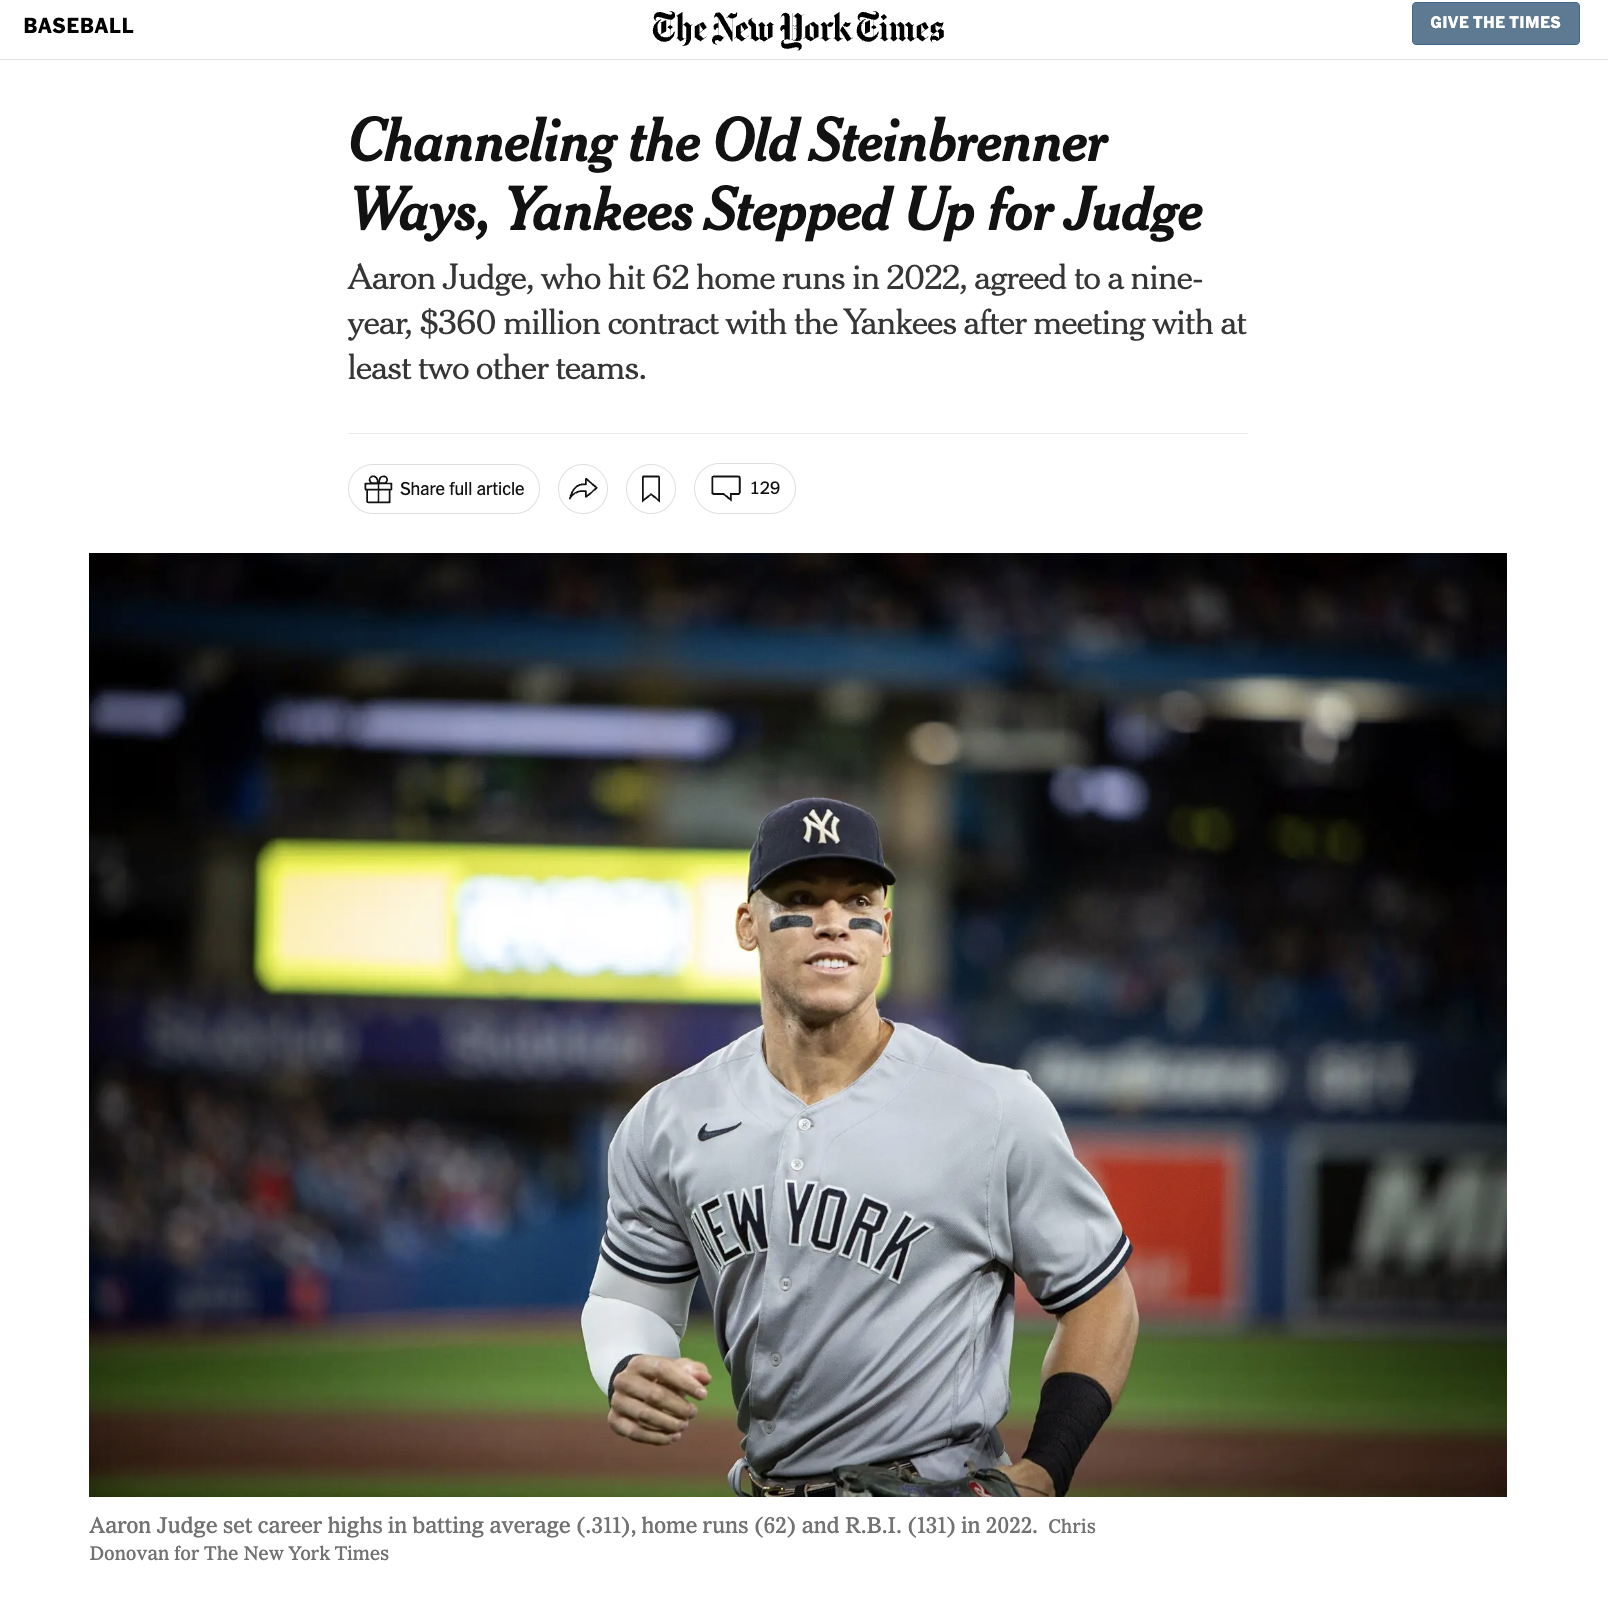
\includegraphics[width = .5\textwidth]{judge}};
\node[anchor = west] at (.5,.5) {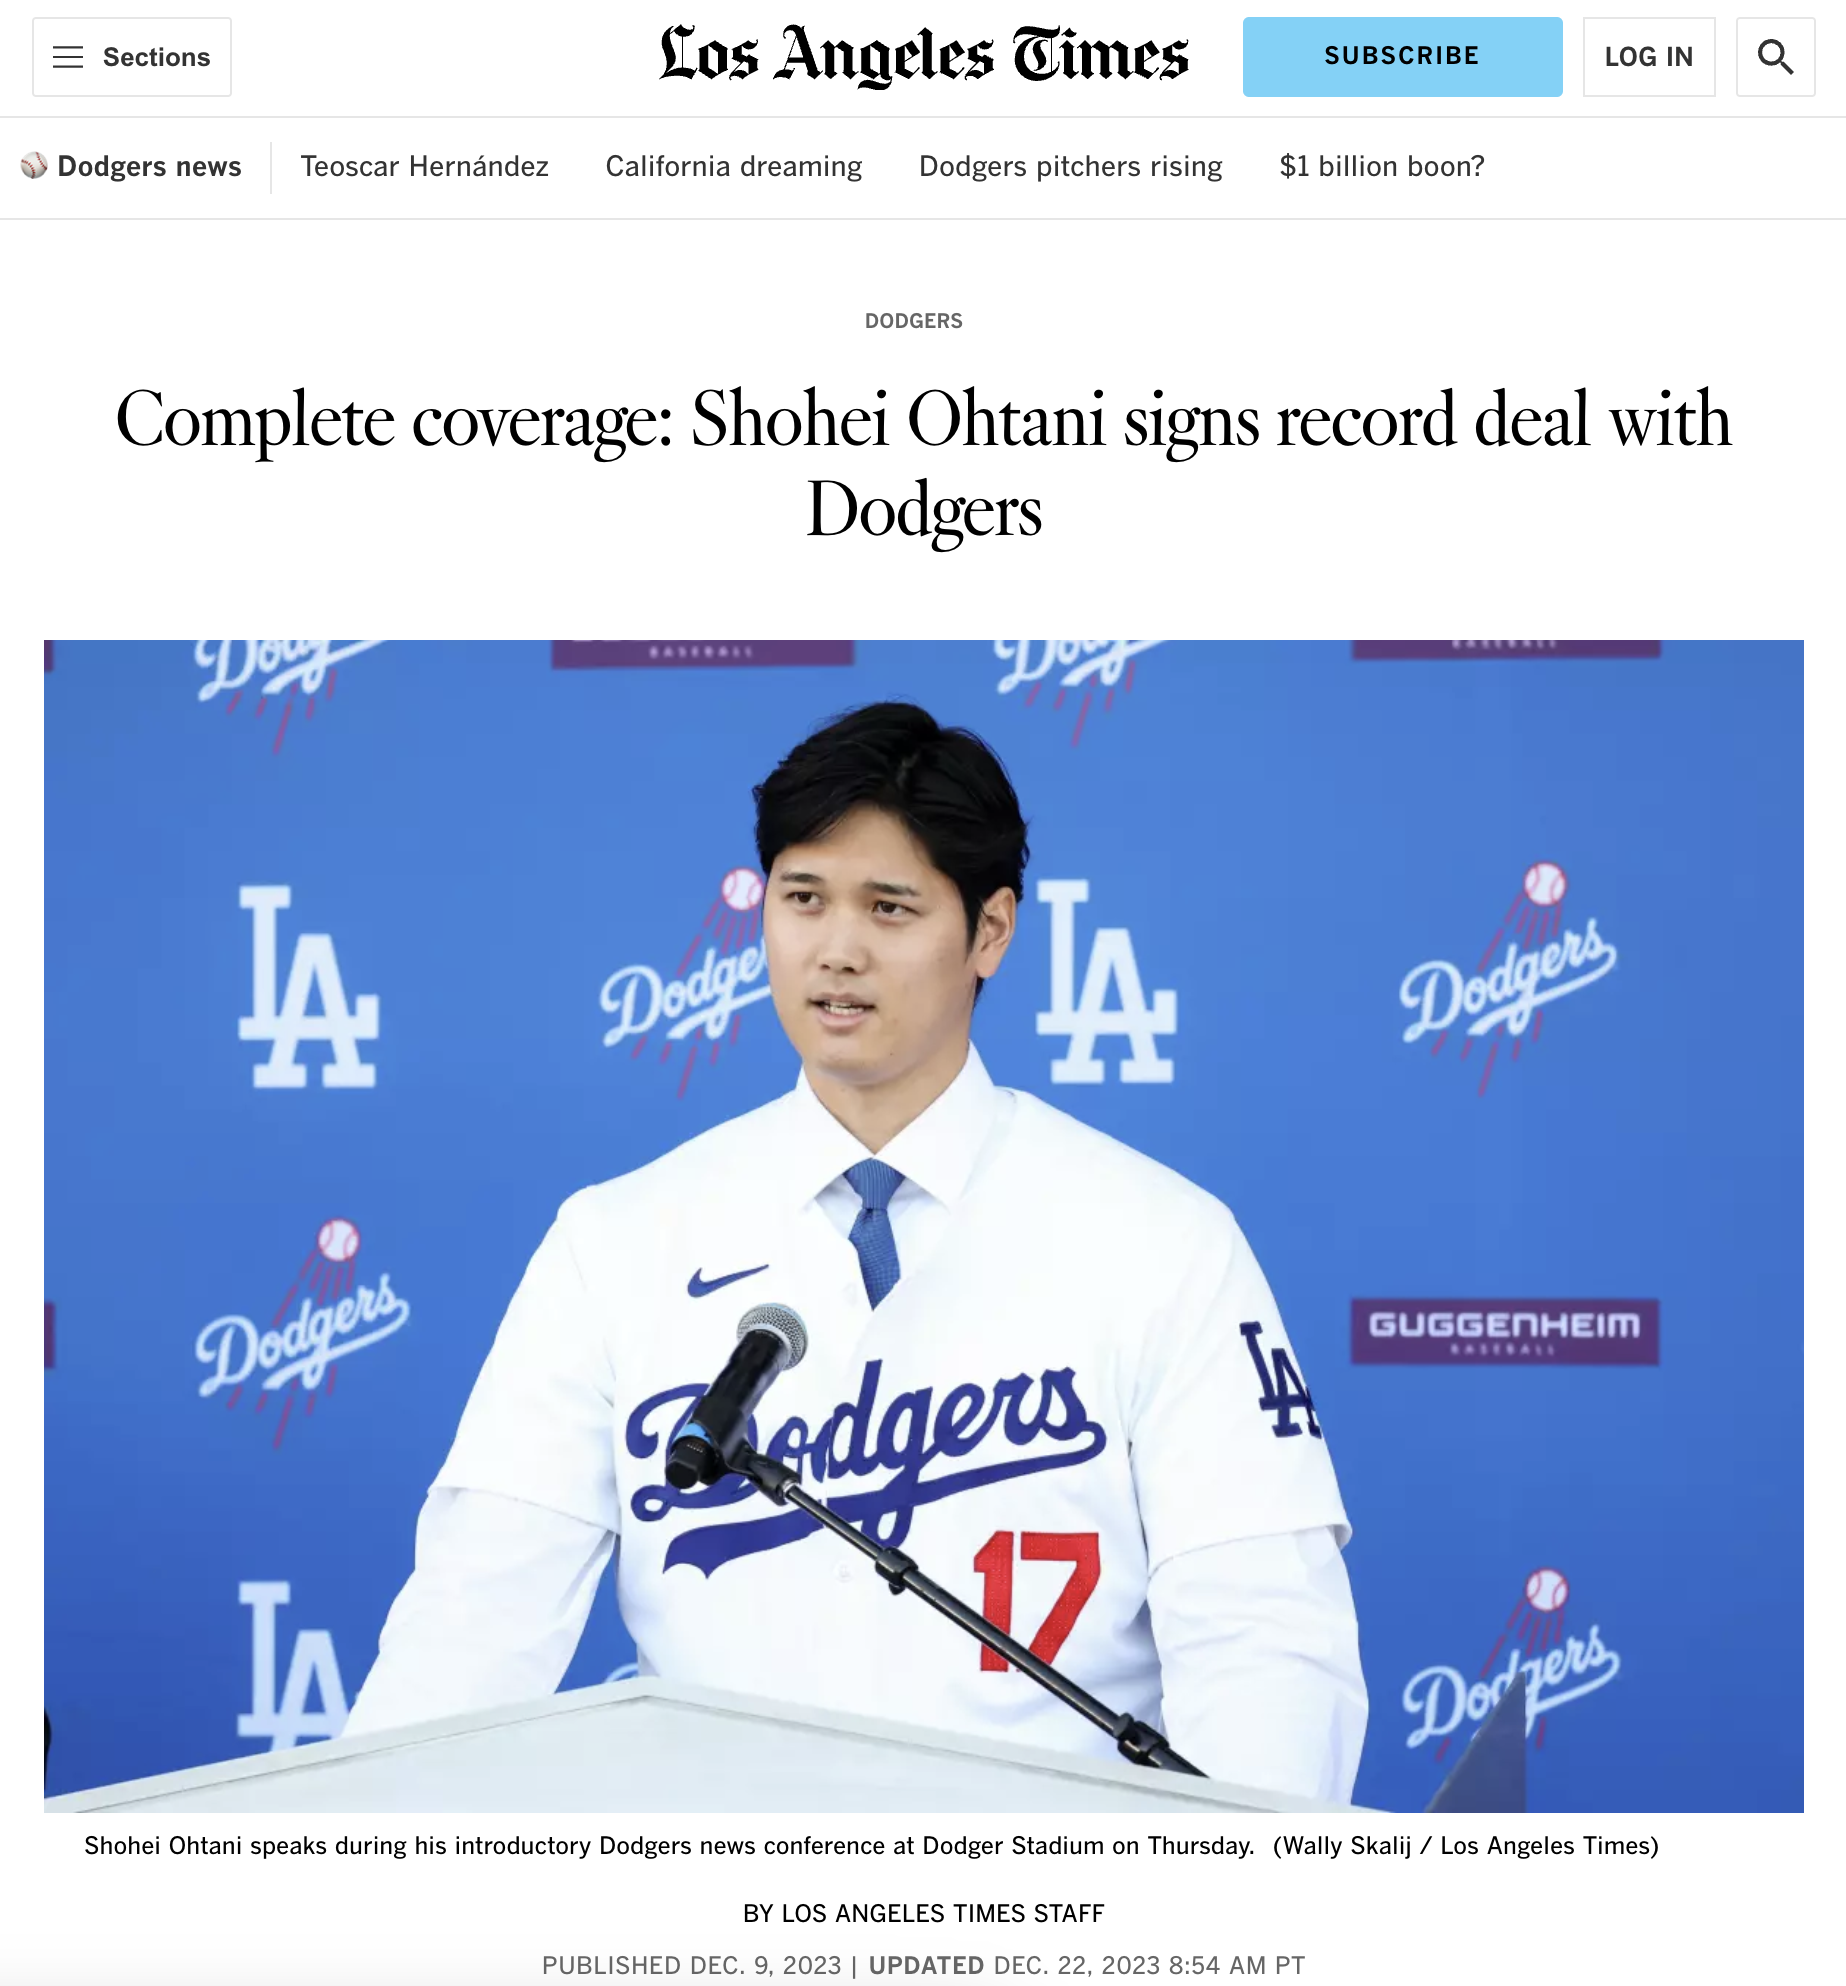
\includegraphics[width = .5\textwidth]{ohtani}};
\node<2->[anchor = north west, align = left, font = \Large] at (0, .1) {Major League Baseball Minimum: \textbf{\$720,000}};
\end{tikzpicture}
\end{frame}

\begin{frame}{Baseball salaries}
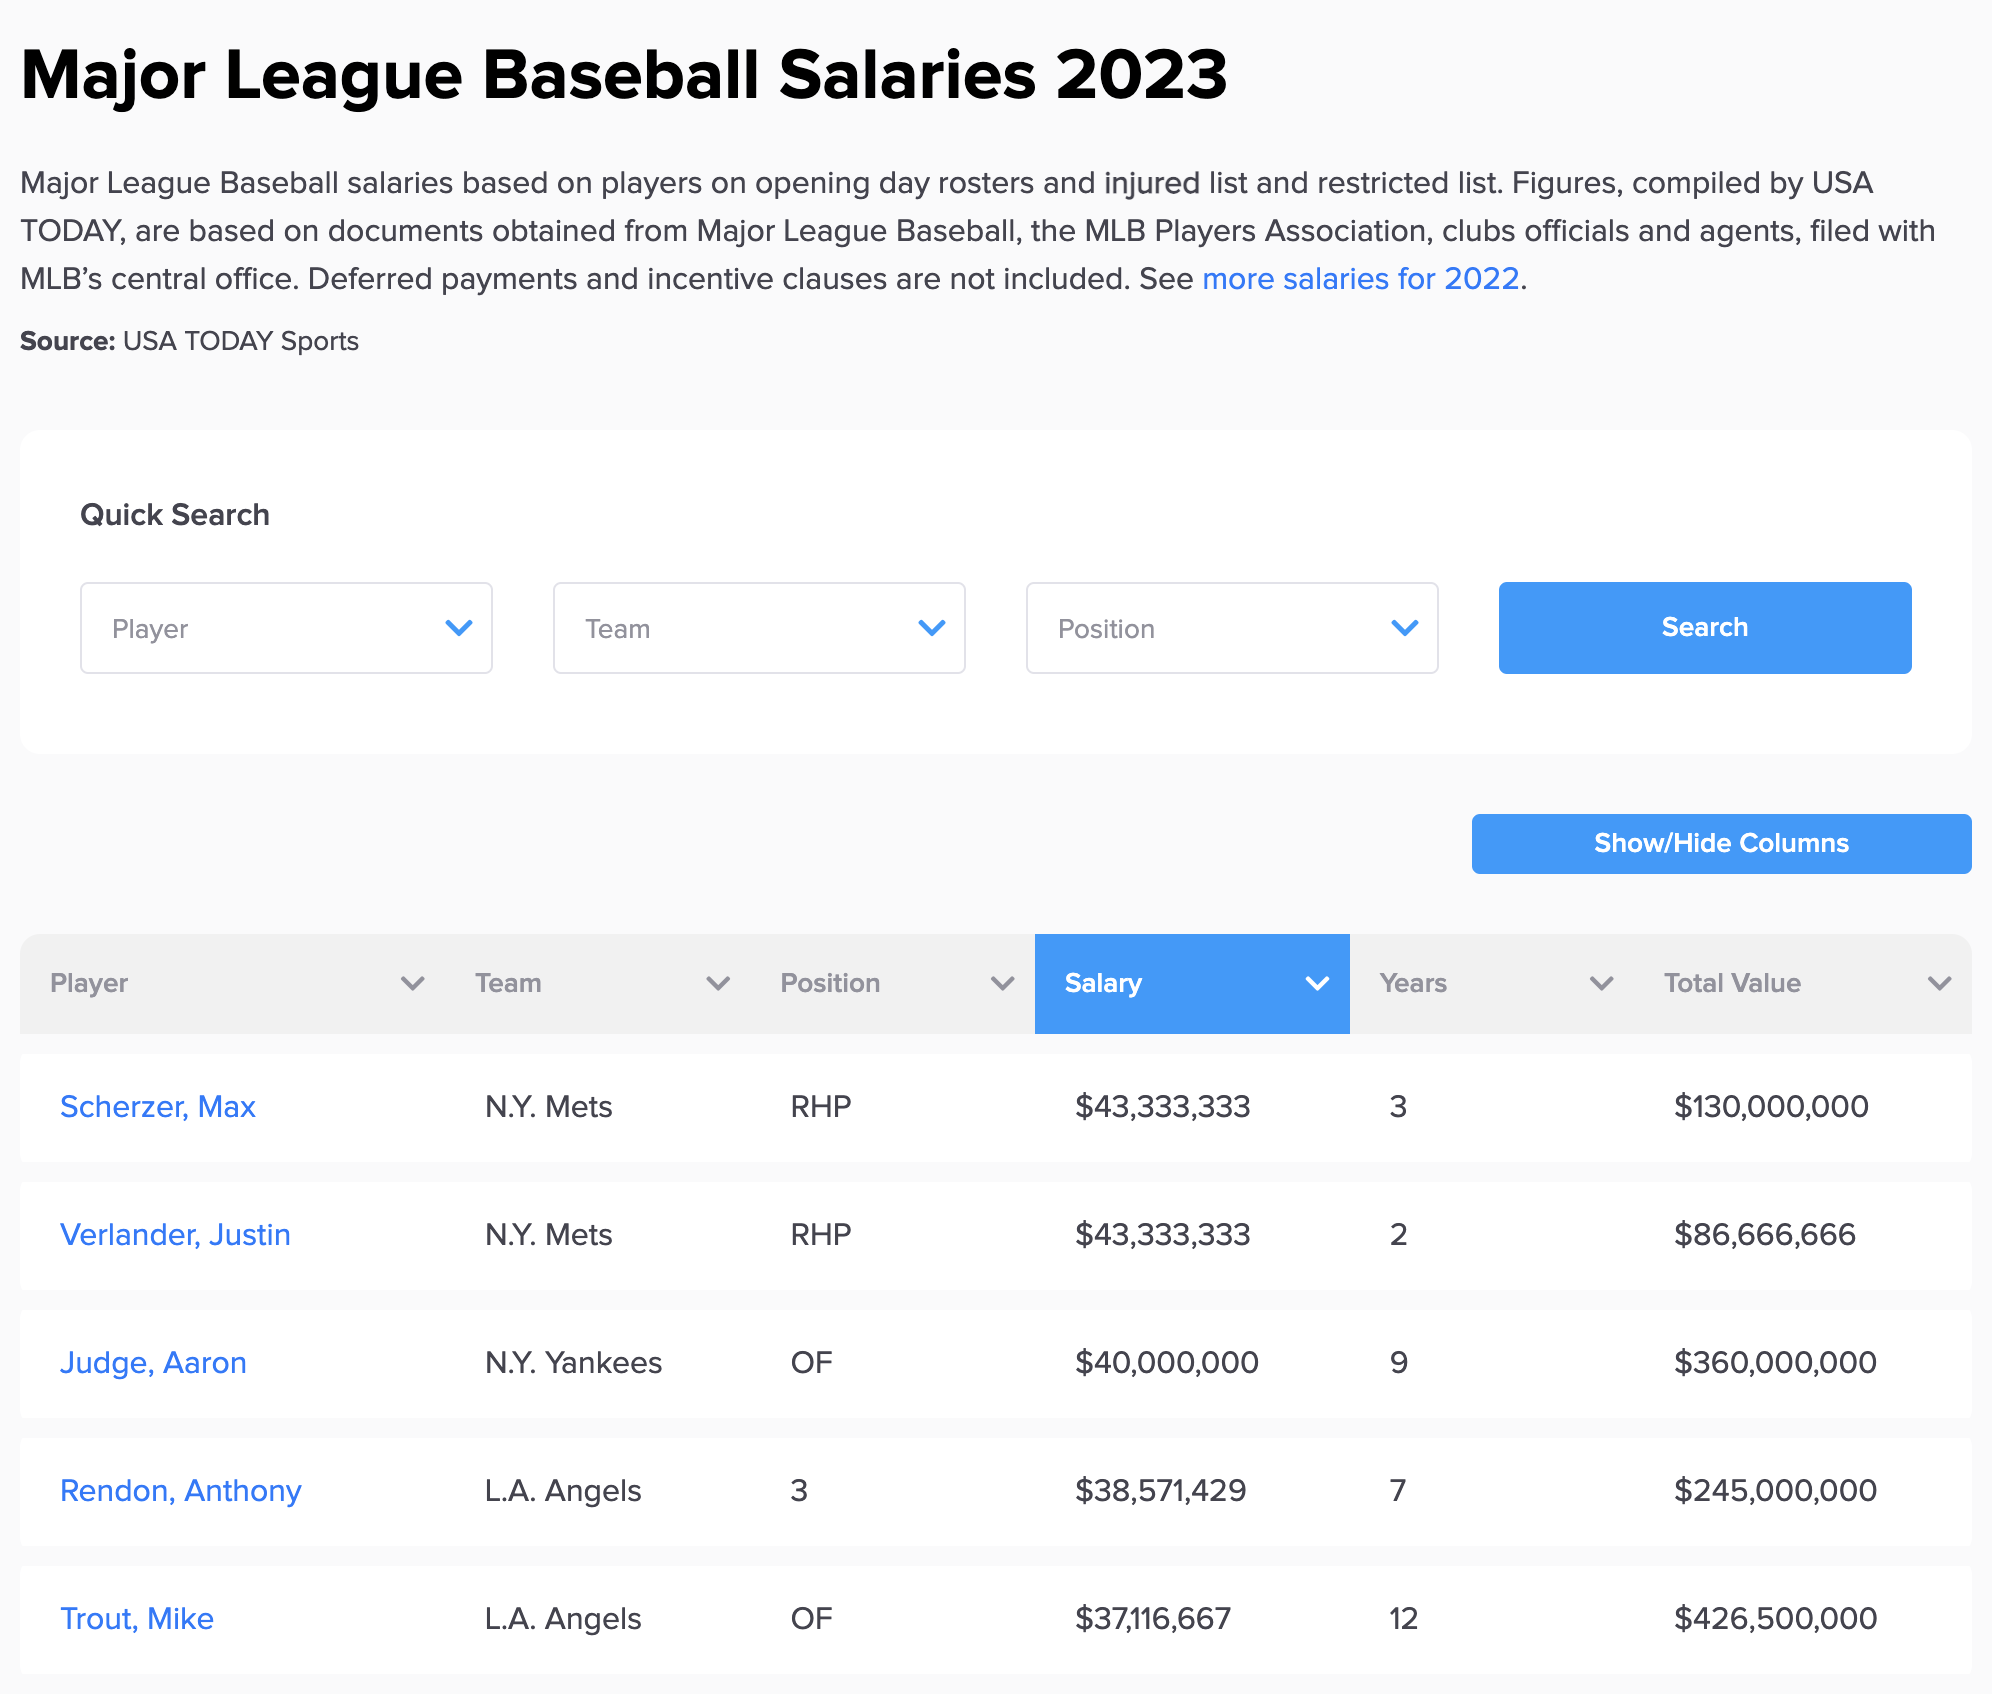
\includegraphics[width = .6\textwidth]{baseball_source}\\
\bref{https://databases.usatoday.com/major-league-baseball-salaries-2023/}{databases.usatoday.com/major-league-baseball-salaries-2023/}
\end{frame}

\begin{frame}{Baseball salaries}
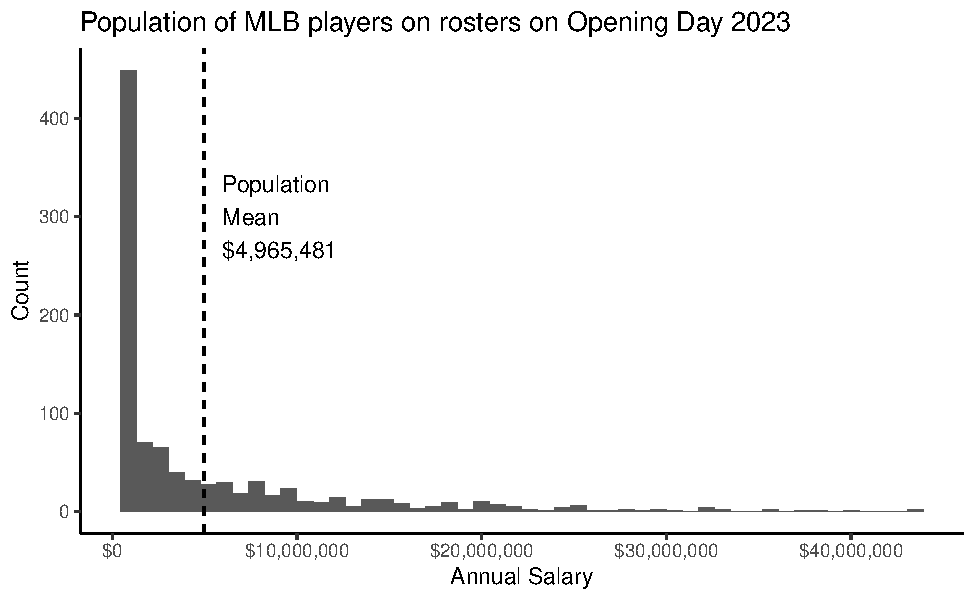
\includegraphics[width = \textwidth]{baseball_histogram}
\end{frame}

\begin{frame}{Baseball salaries}
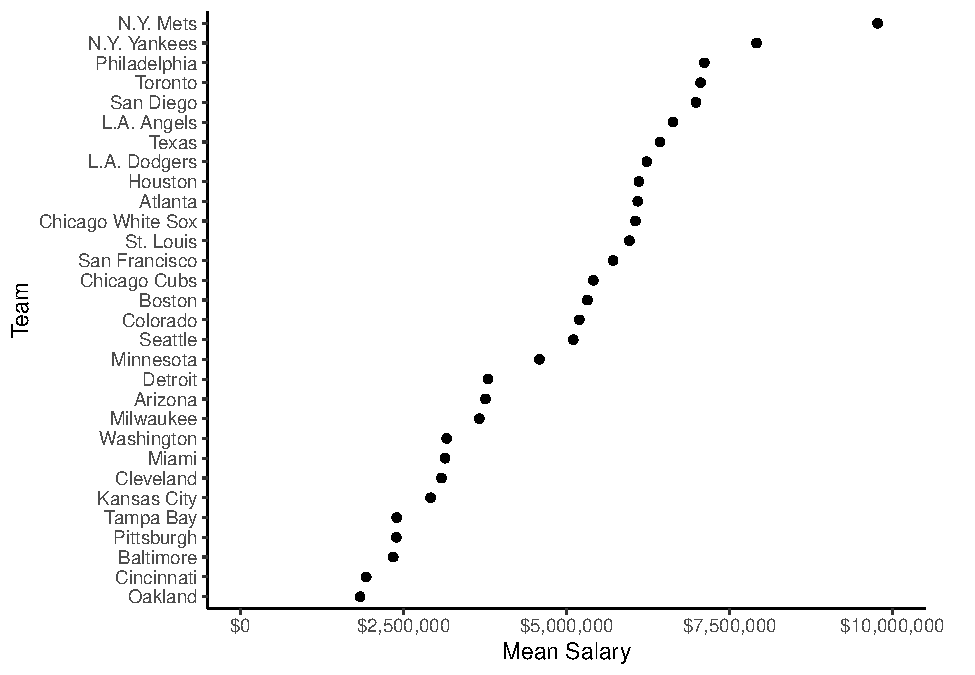
\includegraphics[width = \textwidth]{all_team_mean}
\end{frame}

\section{Draw Samples}

\begin{frame}{Draw a Sample to Estimate the Mean Salary}
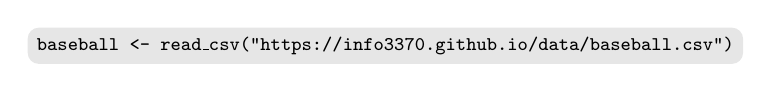
\begin{tikzpicture}
%\node (graph) at (0,0) {\includegraphics[width = .6\textwidth]{baseball_histogram}};
%\node[anchor = west, align = left] at (graph.center) {944 players\\on 30 teams};
%\node[anchor = north west, align = left] at (graph.north east) {Stuck?\\See last week's \bref{https://www150.statcan.gc.ca/n1/edu/power-pouvoir/ch13/prob/5214899-eng.htm}{reading}!};
\node[anchor = north west, font = \scriptsize, fill = gray, fill opacity = .2, text opacity = 1, rounded corners] at (0,0) {\texttt{baseball <- read\_csv("https://info3370.github.io/data/baseball.csv")}};
\end{tikzpicture} \vskip .1in
How would you design:
\begin{itemize}
\item Simple random sample of 60 players
\item Random sample stratified by team
\item Random sample clustered by team
\end{itemize}
and why would you do it each way? \vskip .4in
Stuck? See last week's \bref{https://www150.statcan.gc.ca/n1/edu/power-pouvoir/ch13/prob/5214899-eng.htm}{reading}
\end{frame}

\begin{frame}{Draw a Sample to Estimate the Mean Salary}
\begin{center}
\begin{tabular}{rl}
simple random sampling & 60 players chosen at random \\
stratified sampling & 2 players on each of the 30 teams \\
clustered sampling & 20 players on 3 sampled teams
\end{tabular}
\end{center}
\end{frame}

\section{Apply an Estimator}

\begin{frame}{Apply an Estimator}

Write a function that I like to call \texttt{estimator()}
\begin{itemize}
\item input is a sample
\item output is an estimate
\end{itemize}

\end{frame}


\section{Evaluate Performance}

\begin{frame}{Evaluate performance}

We will first calculate the population mean \vskip .2in

Then we will repeatedly
\begin{itemize}
\item draw a sample
\item apply the estimator
\item store the result
\end{itemize}

\end{frame}

\begin{frame}{Three sampling strategies}
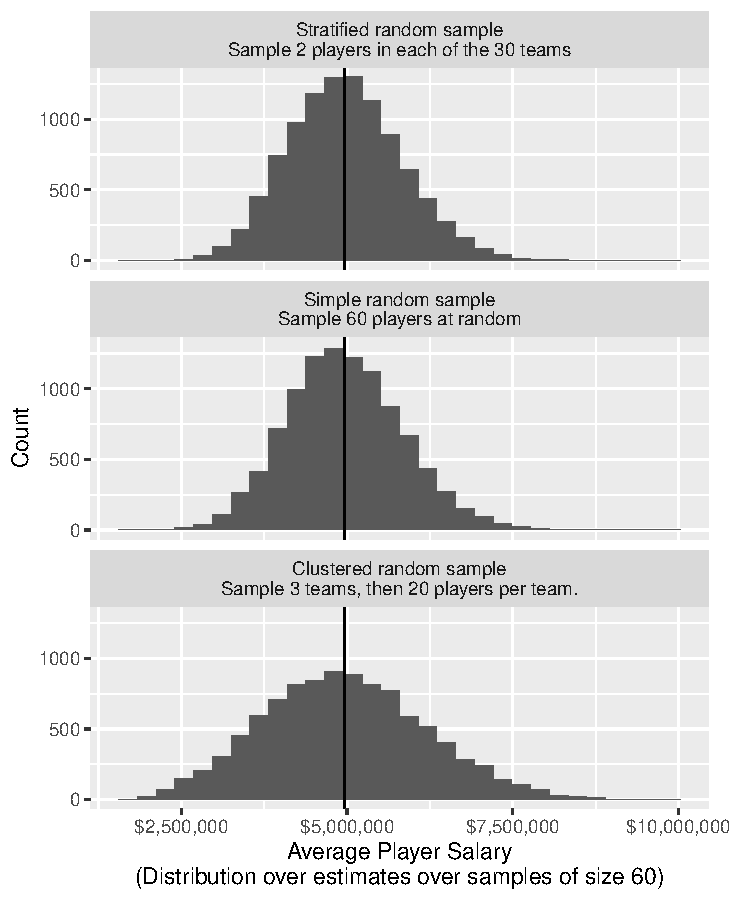
\includegraphics[height = .8\textheight]{baseball_sampling}
\end{frame}

\begin{comment}
\begin{frame}{Sampling: Conclusion}

The baseball players are an unusual example
\begin{itemize}
\item we get to see the whole population
\item we can study the properties of sampling methods
\item usually we just see a sample
\end{itemize} \vskip .1in
Sampling often involves a tradeoff between cost and quality
\begin{itemize}
\item stratified sampling
\begin{itemize}
\item high-quality: guaranteed to get all 30 teams
\item costly: you have to call up all 30 teams!
\end{itemize}
\item simple random sampling
\begin{itemize}
\item a middle ground
\end{itemize}
\item clustered sampling
\begin{itemize}
\item inexpensive: you call only 3 teams!
\item lower quality: risk of 3 unusual teams
\end{itemize}
\end{itemize}

\end{frame}
\end{comment}

\section{Danger of One Sample}

\begin{frame}{Danger of One Sample}

\begin{tikzpicture}[x = \textwidth, y = .8\textheight]
\node at (0,0) {};
\node at (1,1) {};
\node[draw = black, rounded corners, outer sep = 10pt] (population) at (.1,.8) {Population};
\node[draw = black, rounded corners, outer sep = 10pt] (sample) at (.5,.8) {Sample};
\node[draw = black, rounded corners, outer sep = 10pt] (estimate) at (.9,.8) {Estimate};
\draw[->, thick] (population) -- (sample);
\draw[->, thick] (sample) -- (estimate);
\draw[thick] (.3,.68) -- (.3,.75);
\draw[thick] (.3,.38) -- (.3,.43);
\draw[thick] (.7,.68) -- (.7,.75);
\draw[thick] (.7,.38) -- (.7,.43);
\node[outer sep = 10pt, align = center, anchor = north] at (.3, .7) {randomness\\in who is\\chosen};
\node[outer sep = 10pt, align = center, anchor = north] at (.7, .7) {deterministic\\procedures};
\node[outer sep = 10pt, align = center, anchor = north] at (.3, .4) {unavoidable};
\node[outer sep = 10pt, align = center, anchor = north] at (.7, .4) {can be made\\reproducible};
\end{tikzpicture}
\end{frame}

% BEGIN REPRODUCIBILITY

\begin{frame}
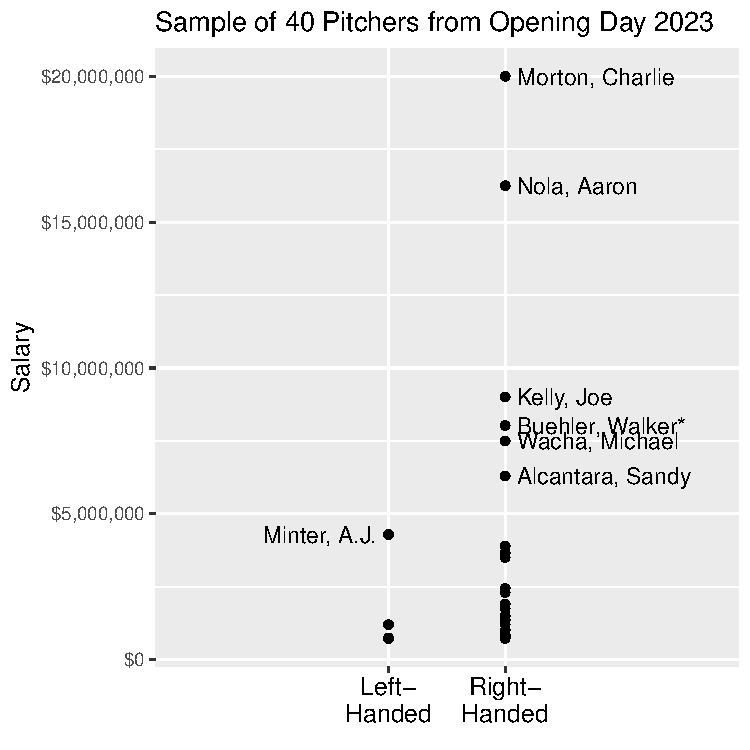
\includegraphics[height = .8\textheight]{baseball_sample}
\end{frame}

\begin{frame}
\begin{tikzpicture}[x = \textwidth, y = \textheight]
\node at (0,0) {};
\node at (1,1) {};
\node at (.5,.5) {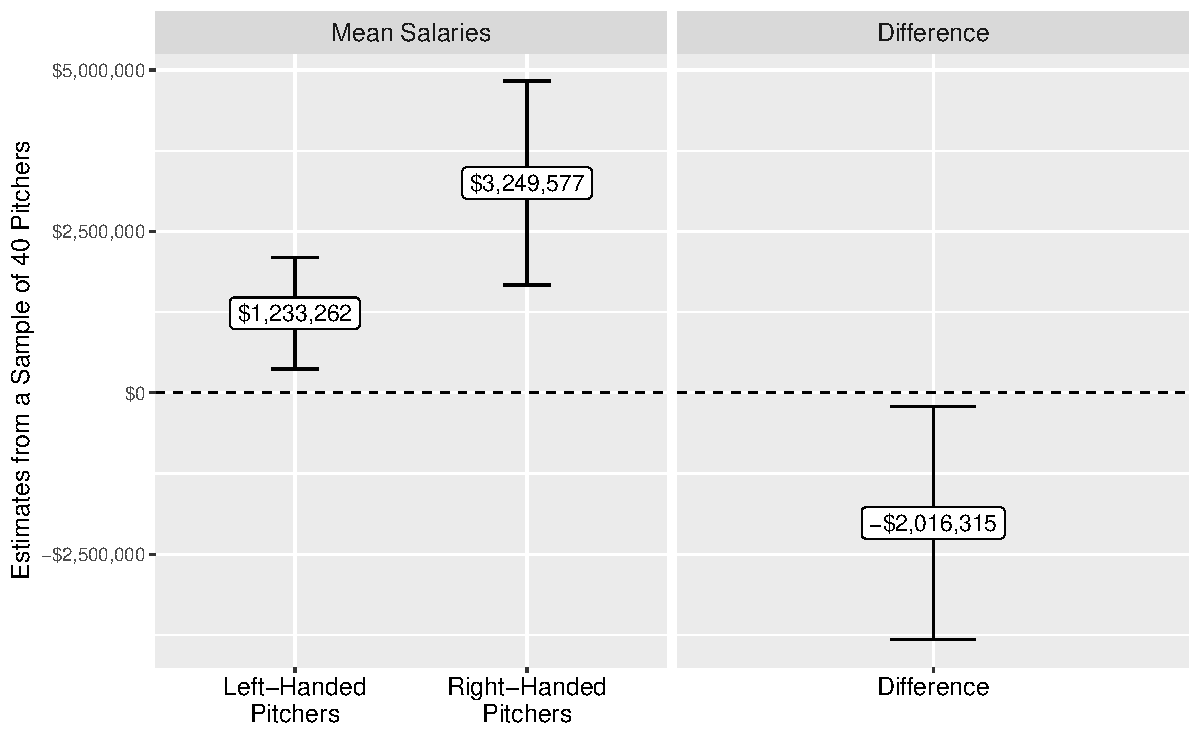
\includegraphics[width = \textwidth]{baseball_one_sample_estimates}};
\draw<1>[white, fill = white] (.56,0) rectangle (1,1);
\node<3->[anchor = north west, font = \large] at (0,.95) {Why might right-handed pitchers earn more?};
\end{tikzpicture}
\end{frame}

\begin{frame}{Your turn}

\begin{itemize}
\item load the data
\item take a sample of size 40
\item group by position
\item summarize the mean salary
\end{itemize} \vskip .2in

Who has higher average salary in your sample?
\begin{itemize}
\item \texttt{RHP}: right-handed pitchers
\item \texttt{LHP}: left-handed pitchers
\end{itemize}

\end{frame}

\begin{frame}
\large
I did this 1,000 times
\end{frame}

\begin{frame}
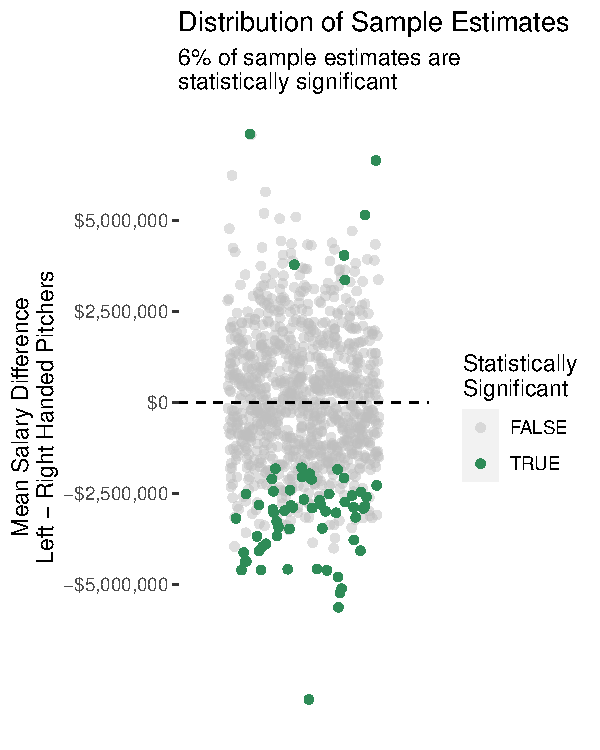
\includegraphics[width = .8\textwidth]{pitchers_sample_scatter}
\end{frame}

\begin{frame}{The replication crisis}

\begin{columns}

\column{.4\linewidth}
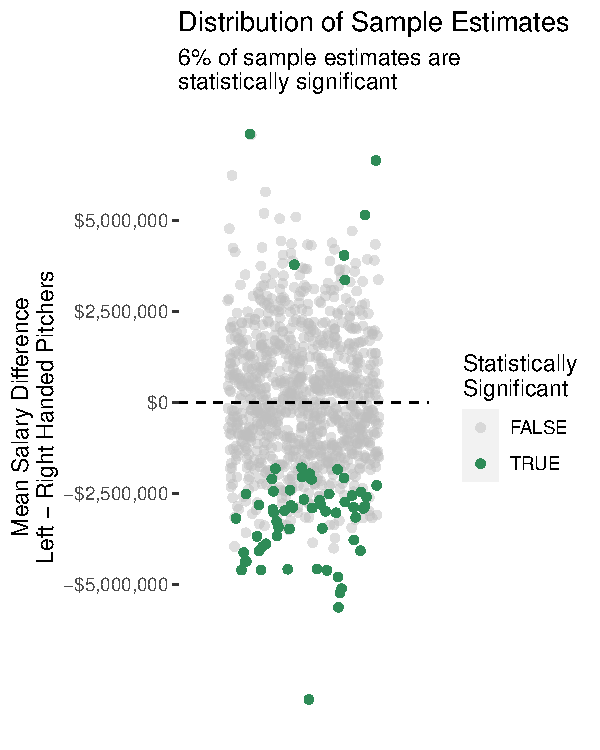
\includegraphics[width = \textwidth]{pitchers_sample_scatter}

\column{.6\linewidth}
\begin{itemize} \pause
\item unless we see the population,\\all estimates involve noise \pause
\item surprising findings yield big rewards \pause
\item unsurprising findings get ignored \pause
\item science is just discovering noise
\end{itemize}

\end{columns}

\end{frame}

\begin{frame}

\includegraphics[width = \textwidth]{bemTitle} \vskip .1in %\pause

\includegraphics[width = \textwidth]{bemSlate}
\bref{https://capture.dropbox.com/ph9Higb0JopbMQe1}{Slate link.}
\end{frame}

\begin{frame}

\includegraphics[width = .48\textwidth]{replication_nhb} %\pause
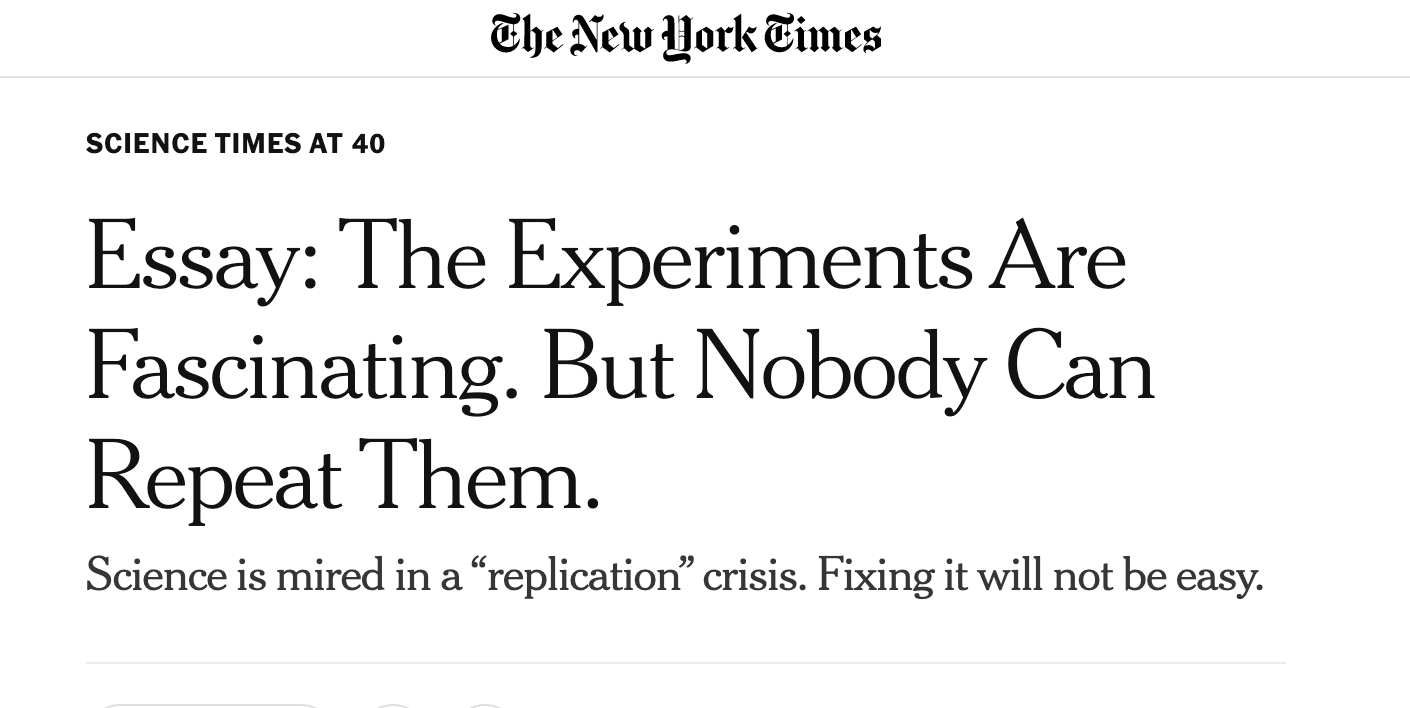
\includegraphics[width = .48\textwidth]{gelmanNyTimes} \vskip .2in
\begin{tiny}
\bref{https://www.nature.com/articles/s41562-018-0399-z}{Camerer et al. in Nature Human Behavior.} \hfill \bref{https://www.nytimes.com/2018/11/19/science/science-research-fraud-reproducibility.html}{Gelman in NYTimes}.
\end{tiny}

\end{frame}

\begin{frame}{The replication crisis}

\begin{columns}

\column{.4\linewidth}
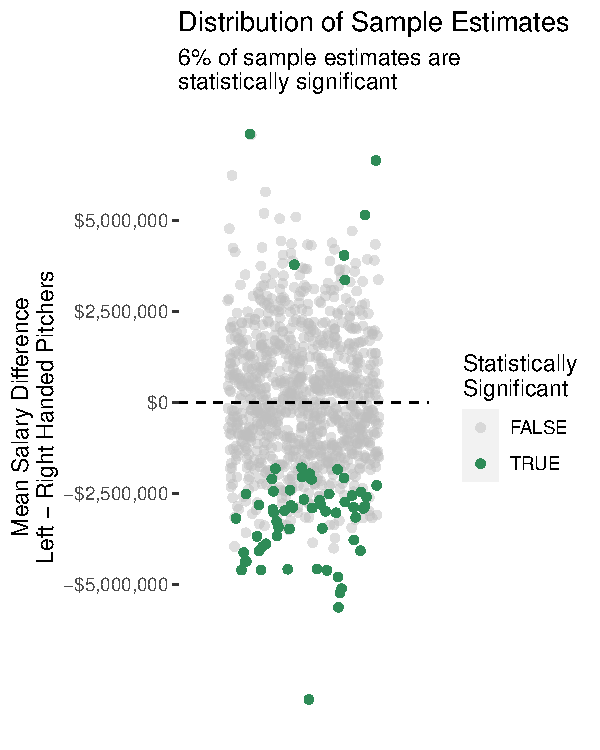
\includegraphics[width = \textwidth]{pitchers_sample_scatter}

\column{.6\linewidth}
\begin{itemize}
\item unless we see the population,\\all estimates involve noise
\item surprising findings yield big rewards
\item unsurprising findings get ignored
\item science is just discovering noise
\end{itemize}

\end{columns}

\end{frame}

\begin{frame}{Danger of One Sample}

\begin{tikzpicture}[x = \textwidth, y = .8\textheight]
\node at (0,0) {};
\node at (1,1) {};
\node[draw = black, rounded corners, outer sep = 10pt] (population) at (.1,.8) {Population};
\node[draw = black, rounded corners, outer sep = 10pt] (sample) at (.5,.8) {Sample};
\node[draw = black, rounded corners, outer sep = 10pt] (estimate) at (.9,.8) {Estimate};
\draw[->, thick] (population) -- (sample);
\draw[->, thick] (sample) -- (estimate);
\draw[thick] (.3,.68) -- (.3,.75);
\draw[thick] (.3,.38) -- (.3,.43);
\draw[thick] (.7,.68) -- (.7,.75);
\draw[thick] (.7,.38) -- (.7,.43);
\node[outer sep = 10pt, align = center, anchor = north] at (.3, .7) {randomness\\in who is\\chosen};
\node[outer sep = 10pt, align = center, anchor = north] at (.7, .7) {deterministic\\procedures};
\node[outer sep = 10pt, align = center, anchor = north] at (.3, .4) {unavoidable};
\node[outer sep = 10pt, align = center, anchor = north] at (.7, .4) {can be made\\reproducible};
\end{tikzpicture}
\end{frame}

\begin{comment}

\begin{frame}{Reproducibility}

provide code so that someone else who has your sample\\can produce your result

\end{frame}

\begin{frame}{Reproducibility}
\includegraphics[height = .5\textheight]{my_code_reproducible}
\end{frame}

\begin{frame}{A bare minimum standard: Reproducibility}
\begin{itemize}
\item does not guarantee credible results
\item but does let us see what created results
\end{itemize}
\end{frame}
\end{comment}

\begin{frame}{Reproducibility}

What is a typical salary in the three highest-paying teams in American baseball? \vskip .1in
\begin{itemize}
\item use the whole population
\item summarize \texttt{salary} grouped by \texttt{team}
\item be ready to tell use your estimates and how you got them
\end{itemize}

\end{frame}

\begin{frame}
What is a typical salary in the three highest-paying teams in American baseball? \vskip .1in \pause
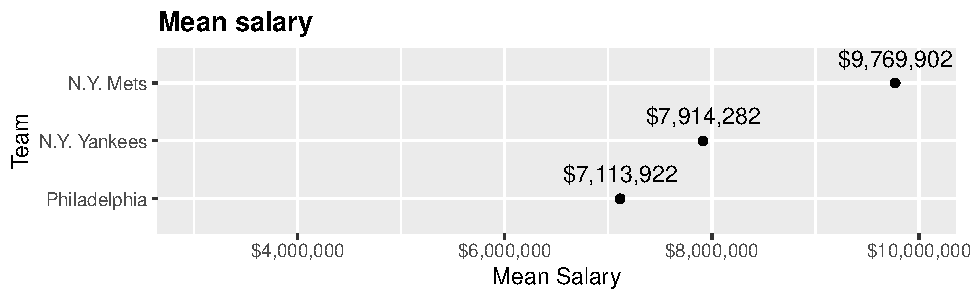
\includegraphics[width = .7\textwidth]{high_team_mean} \vskip .1in \pause
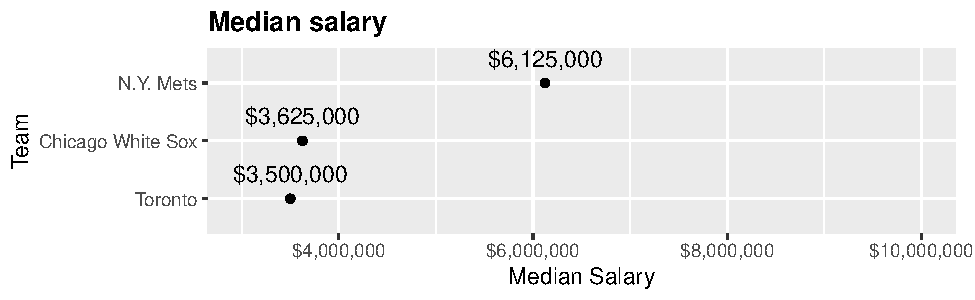
\includegraphics[width = .7\textwidth]{high_team_median} \vskip .1in \pause
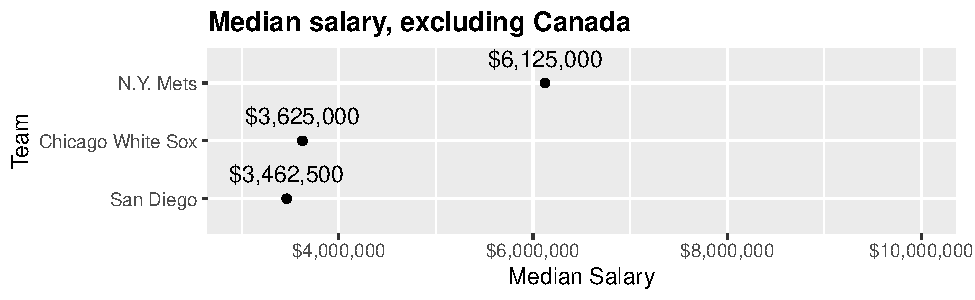
\includegraphics[width = .7\textwidth]{high_team_median_no_canada}
\end{frame}

\begin{frame}

\includegraphics[width = .2\textwidth]{quarto}\\
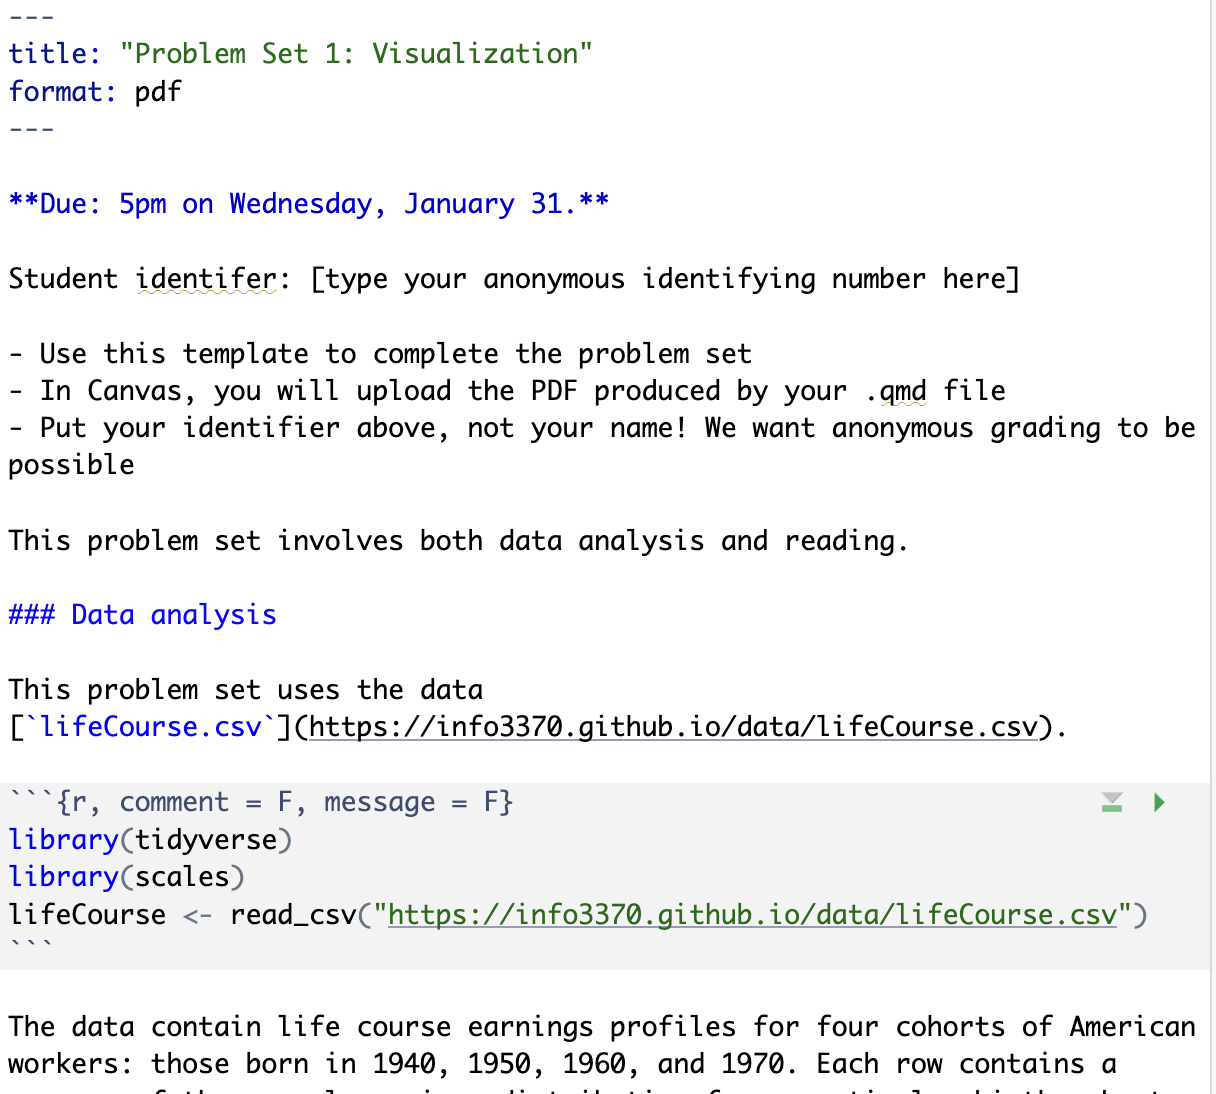
\includegraphics[width = .7\textwidth]{quarto_example}
\end{frame}

\begin{comment}
\begin{frame}{Open problems in reproducibility}
\begin{itemize}
\item sensitivity to software versions
\item sensitivity to operating system
\item computing-intensive research is intensive to replicate
\item privacy and data ethics
\end{itemize}
\end{frame}
\end{comment}

\begin{frame}{Danger of One Sample}
\begin{tikzpicture}[x = \textwidth, y = .8\textheight]
\node at (0,0) {};
\node at (1,1) {};
\node[draw = black, rounded corners, outer sep = 10pt] (population) at (.1,.8) {Population};
\node[draw = black, rounded corners, outer sep = 10pt] (sample) at (.5,.8) {Sample};
\node[draw = black, rounded corners, outer sep = 10pt] (estimate) at (.9,.8) {Estimate};
\draw[->, thick] (population) -- (sample);
\draw[->, thick] (sample) -- (estimate);
\draw[thick] (.3,.68) -- (.3,.75);
\draw[thick] (.3,.38) -- (.3,.43);
\draw[thick] (.7,.68) -- (.7,.75);
\draw[thick] (.7,.38) -- (.7,.43);
\node[outer sep = 10pt, align = center, anchor = north] at (.3, .7) {randomness\\in who is\\chosen};
\node[outer sep = 10pt, align = center, anchor = north] at (.7, .7) {deterministic\\procedures};
\node[outer sep = 10pt, align = center, anchor = north] at (.3, .4) {unavoidable};
\node[outer sep = 10pt, align = center, anchor = north] at (.7, .4) {can be made\\reproducible};
\end{tikzpicture}
\end{frame}

\section{The Future}

\begin{frame}{The Future of Sample Surveys}{Groves, R. M. (2011). \bref{https://doi.org/10.1093/poq/nfr057}{Three eras of survey research.} Public Opinion Quarterly.}

\begin{tikzpicture}[x = \textwidth, y = .6\textheight]
\node at (0,0) {};
\node at (1,1) {};
\onslide<2-8>{
\node[anchor = north west, font = \large] at (0,1) {1930--1960: Era of Invention};
\node<3-4>[anchor = west] (lange) at (0,.5) {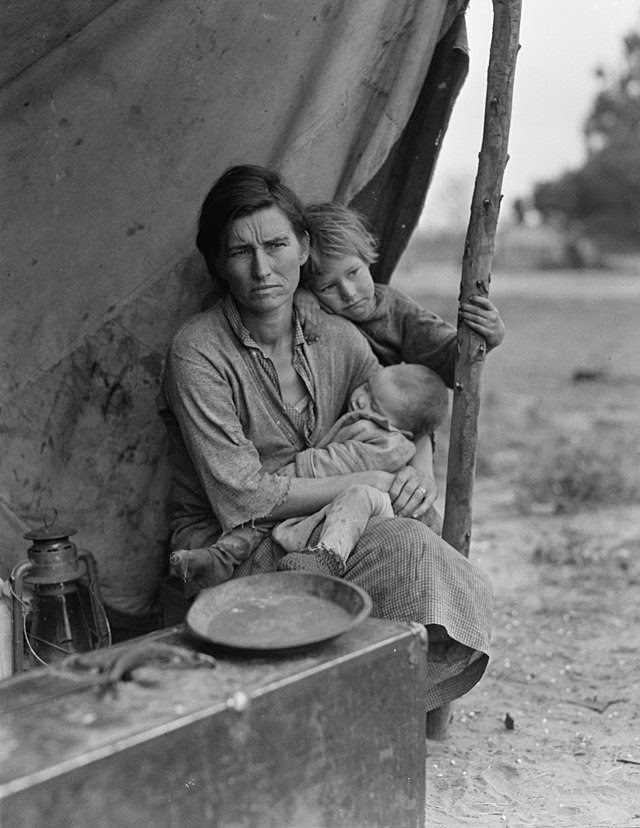
\includegraphics[width = .3\textwidth]{migrantmother}};
\node<4>[anchor = west] at (lange.east)  {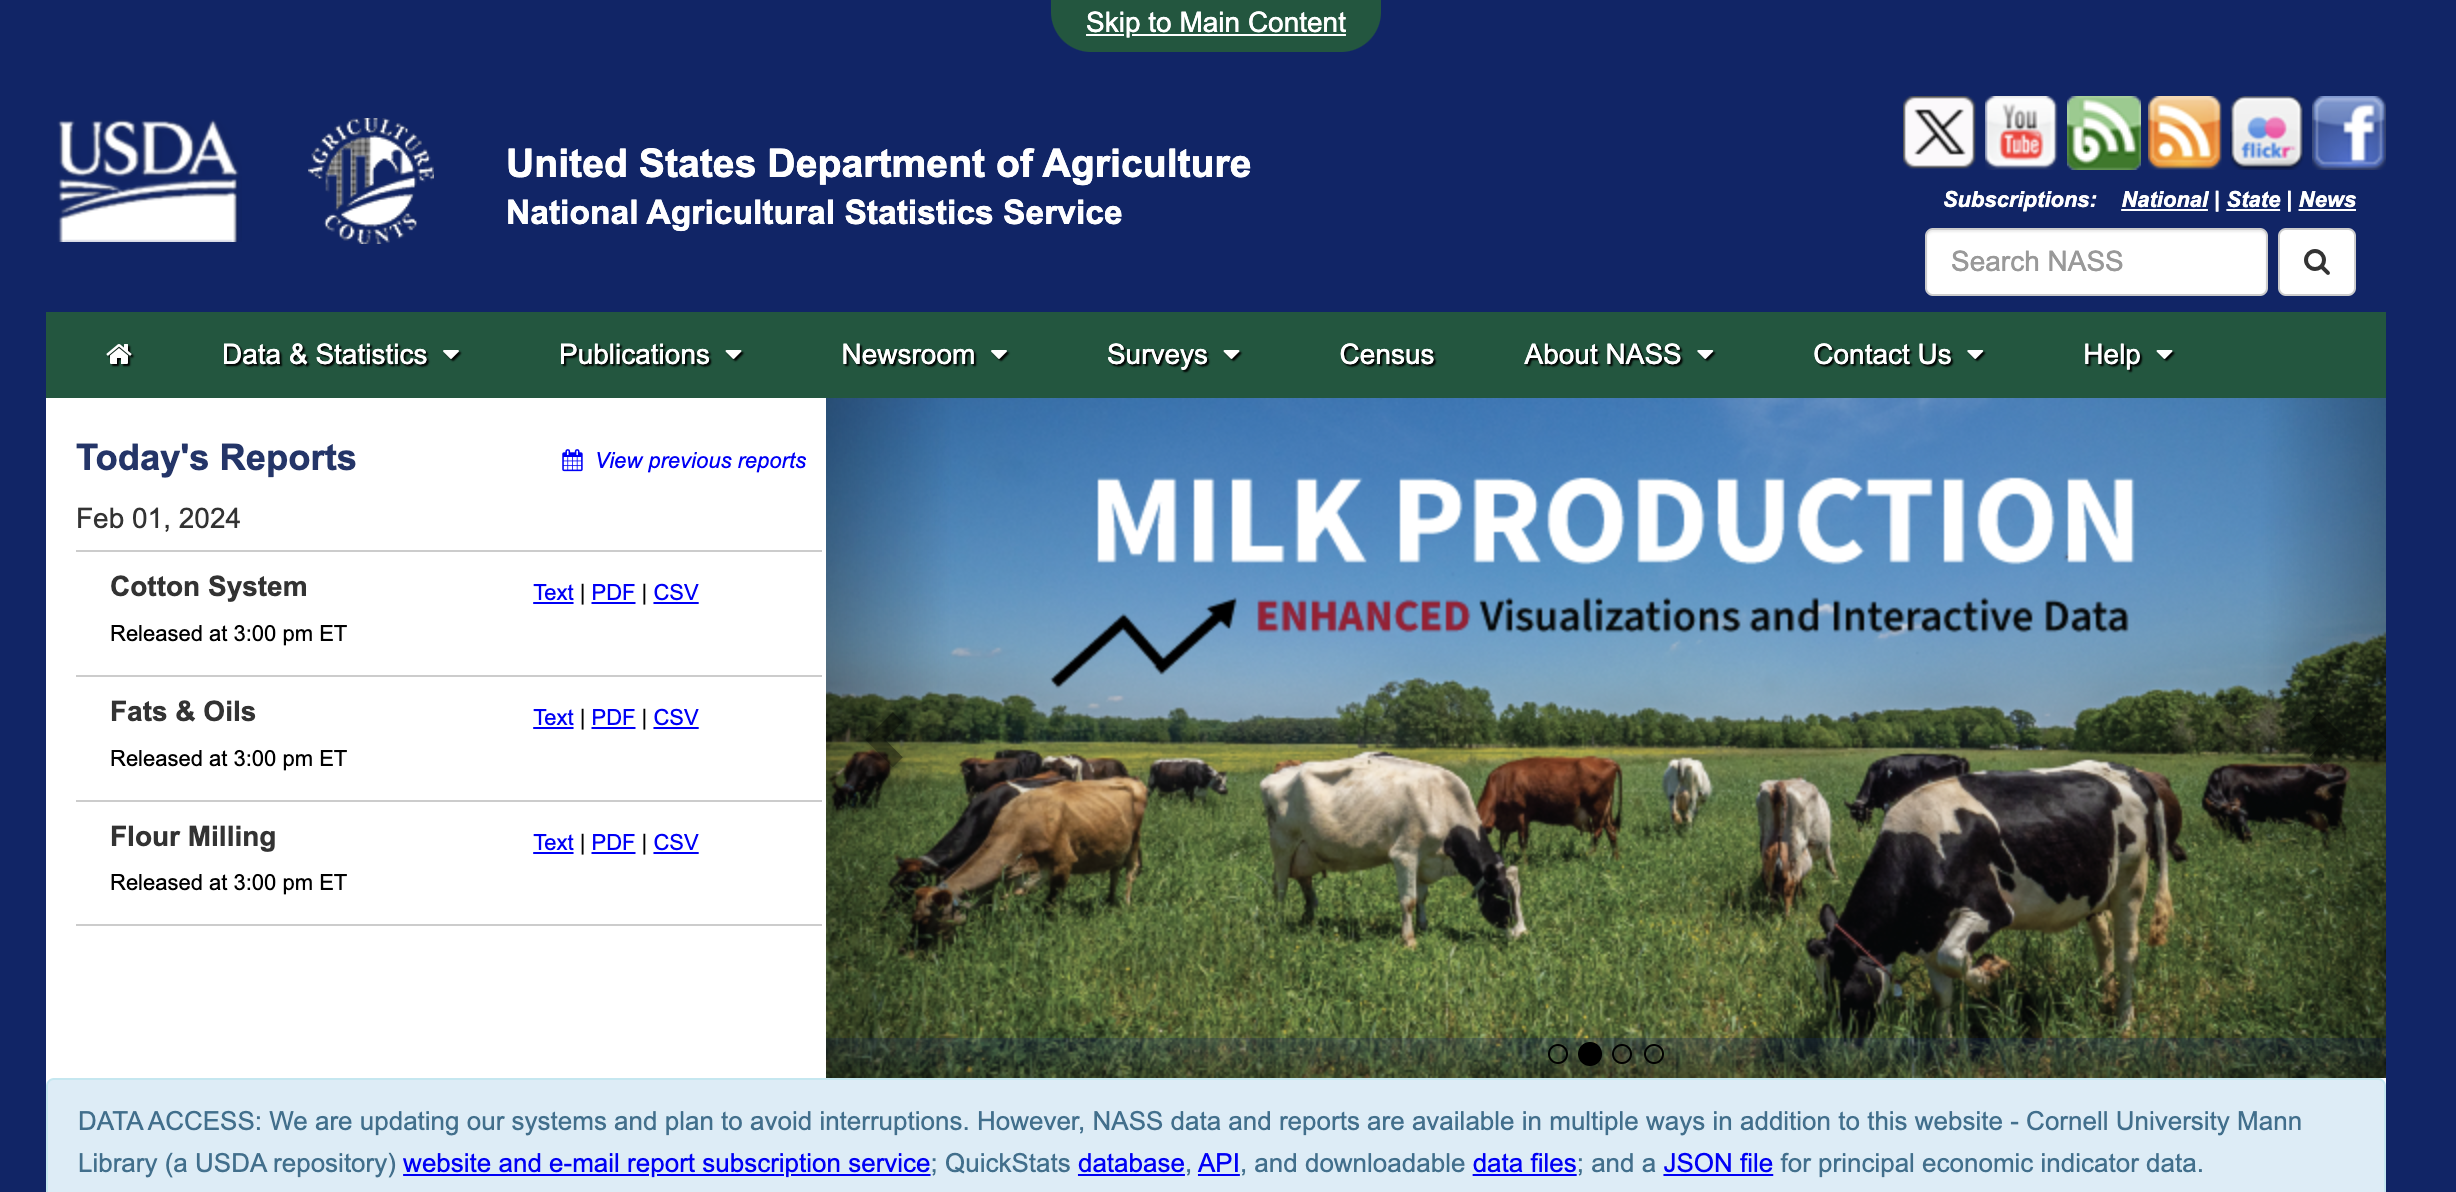
\includegraphics[width = .7\textwidth]{usda}};
\node<5->[anchor = north west] at (0,.7) {sampling frame};
\node<5->[anchor = north west] at (.4,.7) {pieces of land};
\node<6->[anchor = north west] at (0,.6) {mode};
\node<6->[anchor = north west] at (.4,.6) {face-to-face interviews};
\node<7->[anchor = north west] at (0,.5) {cost};
\node<7->[anchor = north west] at (.4,.5) {high};
\node<8->[anchor = north west] at (0,.4) {response rate};
\node<8->[anchor = north west] at (.4,.4) {over 90 percent};
}
\onslide<9-13>{
\node[anchor = north west, font = \large] at (0,1) {1960--1990: Era of Expansion};
\node[anchor = north east] (phone) at (1,1) {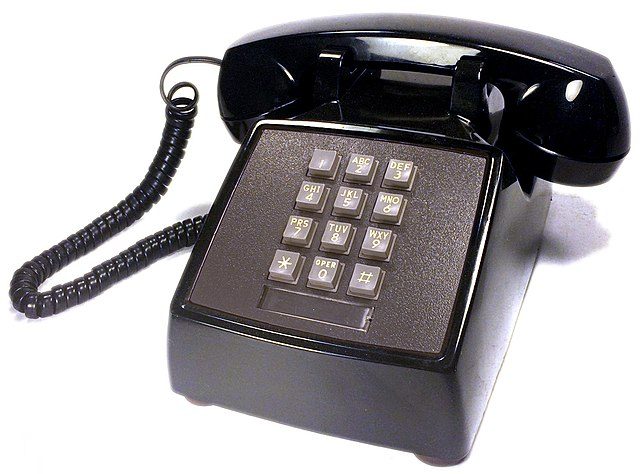
\includegraphics[width = .4\textwidth]{telephone}};
\node[anchor = north east, font = \tiny] at (phone.south east) {Source: \href{https://commons.wikimedia.org/wiki/File:AT\%26T_push_button_telephone_western_electric_model_2500_dmg_black.jpg}{Wikimedia}};
\node[anchor = north west] at (0,.8) {Technology helped: Telephones};
\node<10->[anchor = north west] at (0,.7) {--- sampling frame};
\node<11->[anchor = north west] at (0,.6) {--- mode of data collection};
\node<12->[anchor = north west] at (0,.5) {--- falling costs};
\node<13->[anchor = north west] at (0,.4) {--- falling response rates};
%\node[anchor = north west] at (0,.3) {Computer to aid interviewing and analysis};
}
\onslide<14-19>{
\node[anchor = north west, font = \large] at (0,1) {1990--Present};%: Designed and Organic Data};
\node[anchor = north west] at (0,.85) {Technology brought challenges};
\node<15->[anchor = north west] at (0,.75) {--- answering machines};
\node<16->[anchor = north west] at (0,.65) {--- cell phones};
\node<17->[anchor = north west] at (0,.55) {--- caller ID};
\node<18->[anchor = north west] at (0,.45) {--- response rates plummeted};
\node[anchor = north west] at (.5,.85) {Technology brought opportunities};
\node<19->[anchor = north west] at (.5,.75) {--- digital trace data};
\node<19->[anchor = north west] at (.5,.65) {--- internet panels};
}
\onslide<20->{
\node[anchor = north west, font = \large] at (0,1) {1990--Present: Designed and Organic Data};
\node<21->[anchor = north west] at (0,.85) {Designed data};
\node<21->[anchor = north west] at (.5,.85) {Organic data};
\draw<21-24>[fill = yellow, fill opacity = 1, draw opacity = 0] (.5,.43) -- (.5,.2) -- (.73,.2) -- (.73,.43) -- cycle;
\draw<21-24>[fill = blue, fill opacity = .6, draw opacity = 0] (0,.43) -- (0,.2) -- (.38,.2) --(.38,.2) -- (.38,.43) -- cycle;
\node<22->[anchor = north west] at (0,.75) {--- high cost};
\node<22->[anchor = north west] at (.5,.75) {--- almost free};
\node<23->[anchor = north west] at (0,.66) {--- becoming scarce};
\node<23->[anchor = north west] at (.5,.66) {--- becoming abundant};
\node<24->[anchor = north west] at (0,.57) {--- speak to population};
\node<24->[anchor = north west] at (.5,.57) {--- iffy for population};
\draw<25>[fill = yellow, fill opacity = 1, draw opacity = 0] (.5,.43) -- (.5,.15) -- (.97,.15) -- (1,.2) -- (.97,.25) -- (.73,.25) -- (.73,.43) -- cycle;
\draw<26->[fill = yellow, fill opacity = 1, draw opacity = 0] (.5,.43) -- (.5,0) -- (.97,0) -- (1,.05) -- (.97,.1) -- (.73,.1) -- (.73,.43) -- cycle;
\draw<25->[fill = blue, fill opacity = .6, draw opacity = 0] (0,.43) -- (0,0) -- (.97,0) -- (1,.05) -- (.97,.1) -- (.38,.1) -- (.38,.43) -- cycle;
\draw<26->[fill = green, fill opacity = .6, draw opacity = 0] (.5,.1) -- (.5,0) -- (.97,0) -- (1,.05) -- (.97,.1) -- cycle;
\node<21->[anchor = north west, align = left, color = white] at (0,.43) {\textbf{Example}\\Census age distribution};
\node<21->[anchor = north west, align = left, color = black] at (.5,.43) {\textbf{Example}\\Web histories};
\node<25>[anchor = north east, align = center, black] at (.97,.25) {future of \textbf{organic data}};
\node<25>[anchor = north east, align = center, white] at (.97,.1) {future of \textbf{designed data}};
\node<26->[anchor = north east, align = center, white] at (.97,.1) {the future is \textbf{together}};
}
% 
% Technology: Telephone
% Computer: Analysis and survey flow
% Post-stratification for falling response rates
%
% 1990--Present: Designed and Organic Data
% Answering machines became affordable
% Then cell phones became affordable
% Caller ID
% Internet panels
% "Digital exhaust." Google Flu
\end{tikzpicture}

\end{frame}

\goalsframe

\end{document}






\begin{frame}{Three sampling strategies}

\begin{tikzpicture}[x = \textwidth, y = \textheight]
\node<1>[anchor = north west, align = left] at (0, .15) {1) Which is clustered? Stratified? Simple random sampling?\\2) Walk through how to explain lines of code};
\node<1>[anchor = north west] at (0,.3) {\includegraphics[scale = .25]{read_baseball}};
\node<1>[anchor = north west] at (0,0) {\includegraphics[scale = .25]{strategy_A}};
\node<1>[anchor = north west] at (0,-.2) {\includegraphics[scale = .25]{strategy_B}};
\node<1>[anchor = north west] at (.5,0) {\includegraphics[scale = .25]{strategy_C}};
\node<2>[anchor = north west] at (0,0) {\includegraphics[scale = .5]{strategy_A}};
\node<3>[anchor = north west] at (0,0) {\includegraphics[scale = .5]{strategy_B}};
\node<4>[anchor = north west] at (0,0) {\includegraphics[scale = .4]{strategy_C}};
\end{tikzpicture}

\end{frame}

\begin{frame}
\includegraphics[width = \textwidth]{pitchers_sample_errorbars}
\end{frame}

\begin{frame}
\includegraphics[width = .8\textwidth]{pitchers_sample_hist}
\end{frame}

\begin{frame}{My sample differed from the population by random chance}
\textbf{Population of pitchers}\\
\begin{tabular}{rcc}
& Population & Mean \\
& Size & Salary \\
\hline
Left-handed pitchers 
	& 141
	& 4.3 million \\
Right-handed pitchers
	& 372
	& 4.2 million \\
\end{tabular} \vskip .2in
\textbf{My sample} \\
\begin{tabular}{rcc}
& Sample & Mean \\
& Size & Salary \\
\hline
Left-handed pitchers 
	& 8
	& 1.25 million \\
Right-handed pitchers
	& 32
	& 3.2 million \\
\end{tabular}
\end{frame}
